\section{Hidr�ulica hurbana}
Este trabajo se centra en la implementaci�n de una aplicaci�n en el �rea de hidr�ulica. Es por ello, que es necesario comprender algunos conceptos b�sicos que se describen a continuaci�n:


\subsection{Conceptos de b�sicos de hidr�ulica}
A pesar de que existe una gran diversidad de t�rminos hidr�ulicos, s�lo se describen los estrictamente necesarios para entender el funcionamiento del programa.
\begin{itemize}
	\item \textbf{Presi�n:} Fuerza ejercida sobre una superficie. En este caso se refiere a la fuerza que el agua ejerce durante su recorrido. Generalmente, se expresa como una unidad del  sistema t�cnico a trav�s de metros columna de agua (mca)~\cite{fuertes2002modelacion}.
	\item \textbf{Caudal:} Cantidad de agua que se mueve a trav�s de un segmento de la red. Se expresa en el sistema internacional como metros c�bicos por segundo ($m^3/s$)~\cite{fuertes2002modelacion}.
	% \item \textbf{Factor de fricci�n:} Coeficiente adimensional que especifica la rugosidad de la tuber�a~\cite{Perez-2011}.
	\item \textbf{Curva de consumo:} Patr�n de consumo de agua en un periodo de tiempo. Generalmente el agua es demandada de forma irregular durante el tiempo debido principalmente a las diferentes actividades que la poblaci�n realiza durante el d�a. As�, por ejemplo, el consumo de agua aumenta en los horarios de la ma�ana y tarde~\cite{fuertes2002modelacion}.
\end{itemize}

\subsection{Red de distribuci�n de agua}
Conjunto de elementos enlazados de tal manera que permite suministrar cierta cantidad de agua a una presi�n establecida~\cite{fuertes2002modelacion, Doctoral2012}. En la Figura~\ref{fig:componentesfisicos} se puede apreciar los componentes que conforman la red de agua potable.
% A continuaci�n se define los componentes que conforman una red de agua potable~\cite{Rossman2017}, los cuales se aprecian en la Figura~\ref{fig:componentesfisicos}:

\begin{figure}[h]
	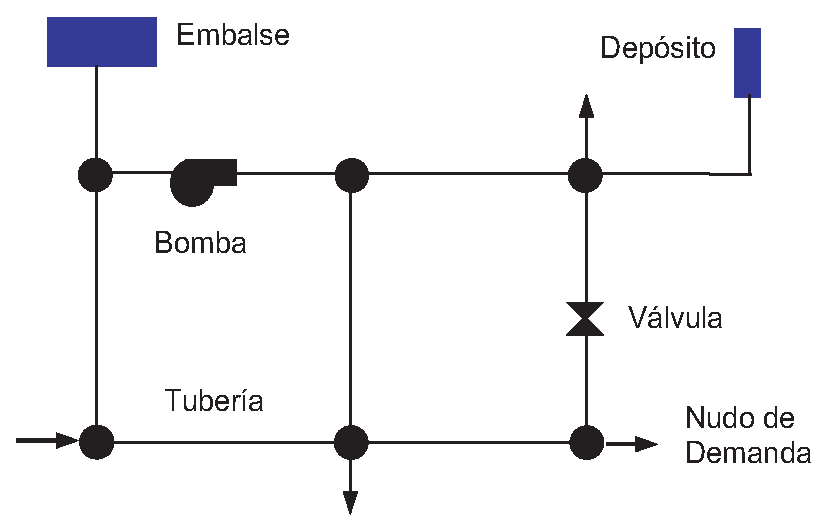
\includegraphics{Capitulo2/assets/componentesfisicosred.eps}
	\centering
	\caption[Componentes f�sicos de un sistema de distribuci�n de agua]{Componentes f�sicos de un sistema de distribuci�n de agua~\cite{Rossman2017}}
	\label{fig:componentesfisicos}
\end{figure}
\subsubsection{Componentes de la red}
\paragraph{Nodos de consumo:} Son puntos de extracci�n de agua. Los niveles de consumo son afectados por la curva de demanda. Cada uno de estos puntos puede requerir diferentes presiones dependiendo de la actividad que genere dicha demanda. En una ciudad, la mayor parte de estos nodos corresponden a viviendas.
\paragraph{Reservorio:} Fuente de alimentaci�n externa desde la que se extrae el agua para alimentar la red, esta fuente puede ser un embalse, un rio, un lago, etc.
\paragraph{Bombas:} Componentes que permiten aportar energ�a al sistema con el fin de impulsar el agua a trav�s de la red. Se encuentran agrupados en estaciones de bombeo. Y su consumo energ�tico representa uno de los costos m�s significativos durante las operaciones en RDA. Por lo tanto, su estudio es verdaderamente importante.
\paragraph{Deposito:} Son elementos con la capacidad de almacenar agua. Generalmente se utilizan para disminuir el trabajo que realizan los equipos de bombeo y permiten aumentar la disponibilidad del recurso en casos de emergencia.
\paragraph{Tuber�as:} Es el medio por el cual transita el agua desde un lugar a otro. Existen diferentes tipos de tuber�as seg�n su material, di�metros y largos. La selecci�n de �stos constituye un problema importante en el dise�o de RDA.
% \paragraph{V�lvulas:} Elementos que limitan la presi�n o el caudal que transita en un punto de la red.